% beautiful title slides in Beamer
% Model 1
% latex-beamer.com

\documentclass[aspectratio=169,xcolor={dvipsnames}]{beamer}

\definecolor{titlesep}{RGB}{243, 156, 17}
\definecolor{white}{rgb}{1,1,1}
\definecolor{tred}{RGB}{244, 67, 54}
\definecolor{tgreen}{RGB}{76, 175, 80}
\definecolor{codebg}{RGB}{38, 50, 56}

\usetheme{metropolis}
% Remove navigation bar
\setbeamertemplate{navigation symbols}{}
\setbeamercolor{frametitle}{fg=white,bg=titlesep}
\setbeamercolor{block title alerted}{use=structure,fg=white,bg=structure.fg!75!Red}
\setbeamercolor{block body alerted}{parent=normal text,use=block title,bg=Melon}

% Tikz package
\usepackage{tikz}
\usetikzlibrary{positioning}
\usepackage{multicol}
\usepackage{multirow}
\usepackage{appendixnumberbeamer}
\usepackage{amsmath}
\usepackage{caption}
\usepackage{subcaption}
\usepackage{minted}
\usepackage{xcolor}
\usepackage{emoji}

\definecolor{strg-color-light}{HTML}{FFC53F}
\definecolor{strg-color-dark}{HTML}{FFA222}
%\definecolor{codebg}{RGB}{38, 50, 56}
%\usemintedstyle{monokai}
\setminted[python3]{breaklines}

\makeatletter

\setlength{\metropolis@progressonsectionpage@linewidth}{1pt}

\ExplSyntaxOn


% marks if title page
\bool_new:N \g_doc_tp_bool
\bool_gset_false:N \g_doc_tp_bool

\AtBeginSection{
    \bool_gset_true:N \g_doc_tp_bool
    \ifbeamer@inframe
      \sectionpage
    \else
      \frame[plain,c,noframenumbering]{\sectionpage}
    \fi
    \bool_gset_false:N \g_doc_tp_bool
}

\setbeamertemplate{background}{%
   \bool_if:NTF \g_doc_tp_bool {
        % title page
        \includegraphics[width=\paperwidth,height=\paperheight]{Background1.png}
   } {
        % non title page
        \includegraphics[width=\paperwidth,height=\paperheight]{Background2.png}
   }

}


\ExplSyntaxOff
\makeatother

\setbeamersize{text margin right=6em}

% Define a new command to switch to a template without a progress bar
\newcommand{\disableprogressbar}{%
  \setbeamertemplate{headline}{} % Remove the headline (which includes the progress bar)
}

% Define a new command to switch back to the original template
\newcommand{\enableprogressbar}{%
  \setbeamertemplate{headline}[default] % Restore the default headline template (with progress bar)
}

\begin{document}
  \begin{frame}[plain]
    %%%%%%%% Title slide details %%%%%%%%%%%%%%


% Background Image
\newcommand{\myBackround}
{
    \includegraphics[width=\paperwidth]{Background1.png}
}

% Title
\newcommand{\myTitle}
{
   ThatMetricTimeline (TMT)
}

% Subtitle
\newcommand{\mySubTitle}
{
    A fully-open source experiment tracking library
}
\newcommand{\repoUrl}
{
    \url{https://github.com/strg-at/strg-events}
}
% Author
\newcommand{\myAuthor}   
{
    Alessio Molinari
}

% Affiliation
\newcommand{\myAffiliate}
{
    %\textsuperscript{1}ISTI-CNR, \textsuperscript{2}University of Pisa
 % Affiliation here
}

% Presentation Date
\newcommand{\myDate}   
{
    %\today
    April 12, 2024
}

%%%%%%%%%%%%%%%%%%%%%%%%%%%%%%%%%%%%


%%%%%%%%%% Title slide code %%%%%%%%%%%
\begin{tikzpicture}[remember picture,overlay]


% Background image
\node[above right,inner sep=0pt] at (current page.south west)
    {
        \myBackround
    };
    
% Title & Subtitle
\node
[
    above right=1.5cm and 3cm,
    anchor=east,
    align=center,
    %fill=strg-color-light,
    text=strg-color-dark,
    rounded corners,
    inner xsep=15pt,
    inner ysep=10pt, 
    minimum width=0.7\textwidth,
    text width=0.6\textwidth
] (title) at (current page.center)
{
    \LARGE \myTitle  \\[5pt]
    \small \mySubTitle
};

% repo URL
\node[below=0.8cm,text=strg-color-dark] (url) at (title.south){
    \small \repoUrl
};

% Author 
\node[below right=3.8cm and 1cm, text=white] (author) at (title.south east){\myAuthor};

% Date
\node[below=0.01mm, text=white] (date) at (author.south){\myDate};

\end{tikzpicture}
  \end{frame}

  \section{About me \emoji{man-raising-hand}}
  \begin{frame}{About me}
    Just a quick glance at my history:
    \begin{itemize}
      \item I'm originally from Rome, Italy \emoji{pinched-fingers}
      \item Got my Master degree and later PhD in Pisa, Italy \emoji{man-student}
      \item Now I work at STRG.at \emoji{technologist}
      \item I'm a Linux and open source enthusiast \emoji{penguin}
    \end{itemize}
  \end{frame}

  \begin{frame}{About me: OSS contributions}
    In general, I enjoy contributing to OS software. Most relevant contributions are to:
    \begin{itemize}
      \item the \texttt{Hyprland} compositor (Contributor, \url{https://github.com/hyprwm/Hyprland});
      \item the \texttt{hyprland-virtual-desktops} plugin (Author, \url{https://github.com/levnikmyskin/hyprland-virtual-desktops});
      \item minor contributions to Telegram, Waybar, and many other projects I don't remember anymore;
    \end{itemize}
  \end{frame}

  \section{That Metric Timeline: why?}
  \begin{frame}{TMT: Background}
    When working on a research project, experiments, their results
    and the code that generated them can easily get lost:
    \begin{itemize}
      \item git is not a solution, we don't commit every time we change a hyperparameter;
      \item some solutions were available, but they were overly complicated, or not open source;
    \end{itemize}
  \end{frame}
  \begin{frame}{TMT: Background}
    I wanted something that was:
    \begin{itemize}
      \item truly open source (read, you can contribute);
      \item simple (following KISS);
    \end{itemize}
    Where KISS means that \texttt{tmt} should be a simple software, with no unnecessary architectures,
    interfaces etc.\\Even if this means the user needs to write their own little scripts around it.
  \end{frame}

  \section{That Metric Timeline: what?}
  \begin{frame}{TMT: what is it?}
    \texttt{tmt} (\url{https://github.com/levnikmyskin/that_metric_timeline}) is a Python library which:
    \begin{itemize}
      \item keeps a local ``database'' of your experiments, with names, descriptions, metrics etc;
      \item keeps local snapshots of the code that generated those experiments;
      \item is fully open source, fully offline, terminal-centric (read, you can run it on your servers);
    \end{itemize}
  \end{frame}
  \begin{frame}{TMT: snapshots}
    Code snapshots between different runs are created by:
    \begin{itemize}
      \item hardlinking all files that didn't change since last snapshot;
      \item copying only files that changed
    \end{itemize}
    Basically, this is to avoid your local storage explodes when you're convinced that 
    \\those two layers are to blame for such a low F1, and you're determined to try all possible 
    combinations by hand.
  \end{frame}
  \begin{frame}{TMT: local database}
    \texttt{tmt} local ``database'' is actually a bunch of \texttt{json} files stored
    in the \texttt{.tmt} folder at\\the root of your repository.\\
    You can simply read those files, but \texttt{tmt} exposes a few utilities to deal with them.
  \end{frame}

  \section{TMT: tracking your experiments}
  \begin{frame}[fragile]{TMT: tracking your experiments}
      \begin{minted}{python3}
        from tmt import tmt_recorder

        @tmt_recorder(name="some_experiment")
        def train_and_predict(x_tr, y_tr, x_te, y_te):
            lr = LogisticRegression()
            lr.fit(x_tr, y_tr)
            preds = lr.predict(x_te)
            return {
              'f1': f1_score(y_te, preds), 
              'accuracy': accuracy_score(y_te, preds)
            }
      \end{minted}
  \end{frame}
  \begin{frame}[fragile]{TMT: tracking your experiments}
    \begin{minted}[highlightlines={3,7}]{python3}
      from tmt import tmt_recorder, tmt_save

      @tmt_recorder(name="some_experiment_with_data", description="saving preds this time")
      def train_and_predict(...):
        ...
        preds = lr.predict(x_te)
        tmt_save(preds, name='lr_predictions')
        return {
          'f1': f1_score(y_te, preds), 
          'accuracy': accuracy_score(y_te, preds)
        }
    \end{minted}
  \end{frame}

  \section{TMT: searching and loading your experiments \emoji{magnifying-glass-tilted-right}}
  \begin{frame}{TMT: the TUI interface}
   \begin{figure}
    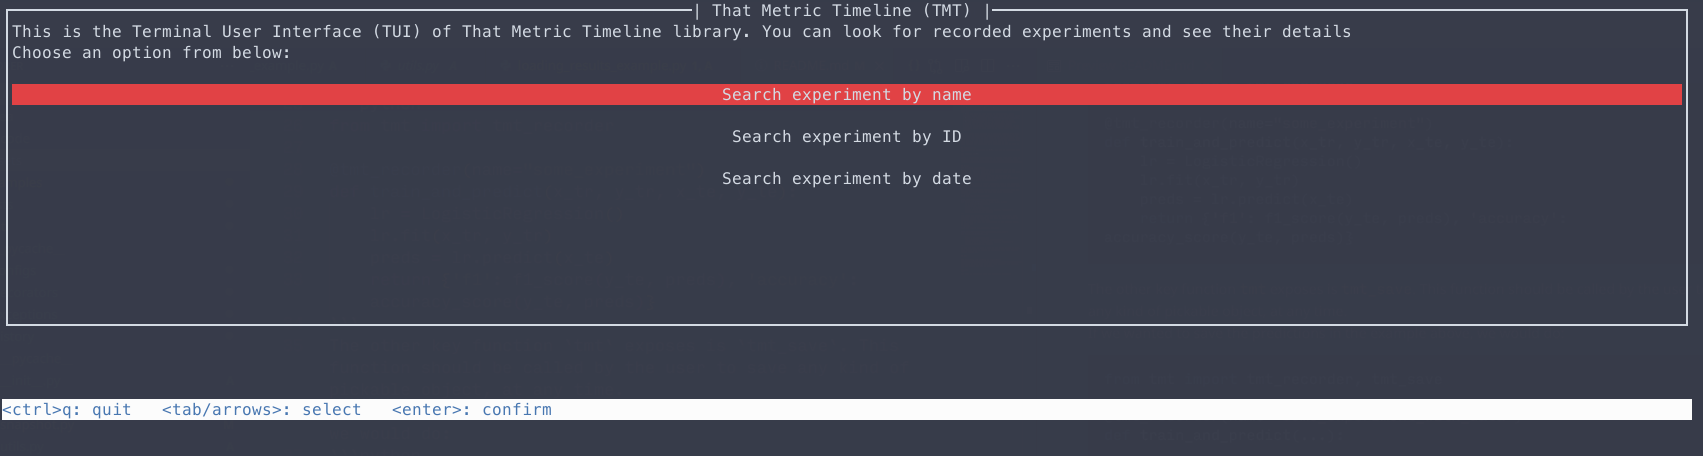
\includegraphics[width=0.90\textwidth]{main_tui.png}
   \end{figure} 
  \end{frame}
  \begin{frame}{TMT: the TUI interface}
   \begin{figure}
    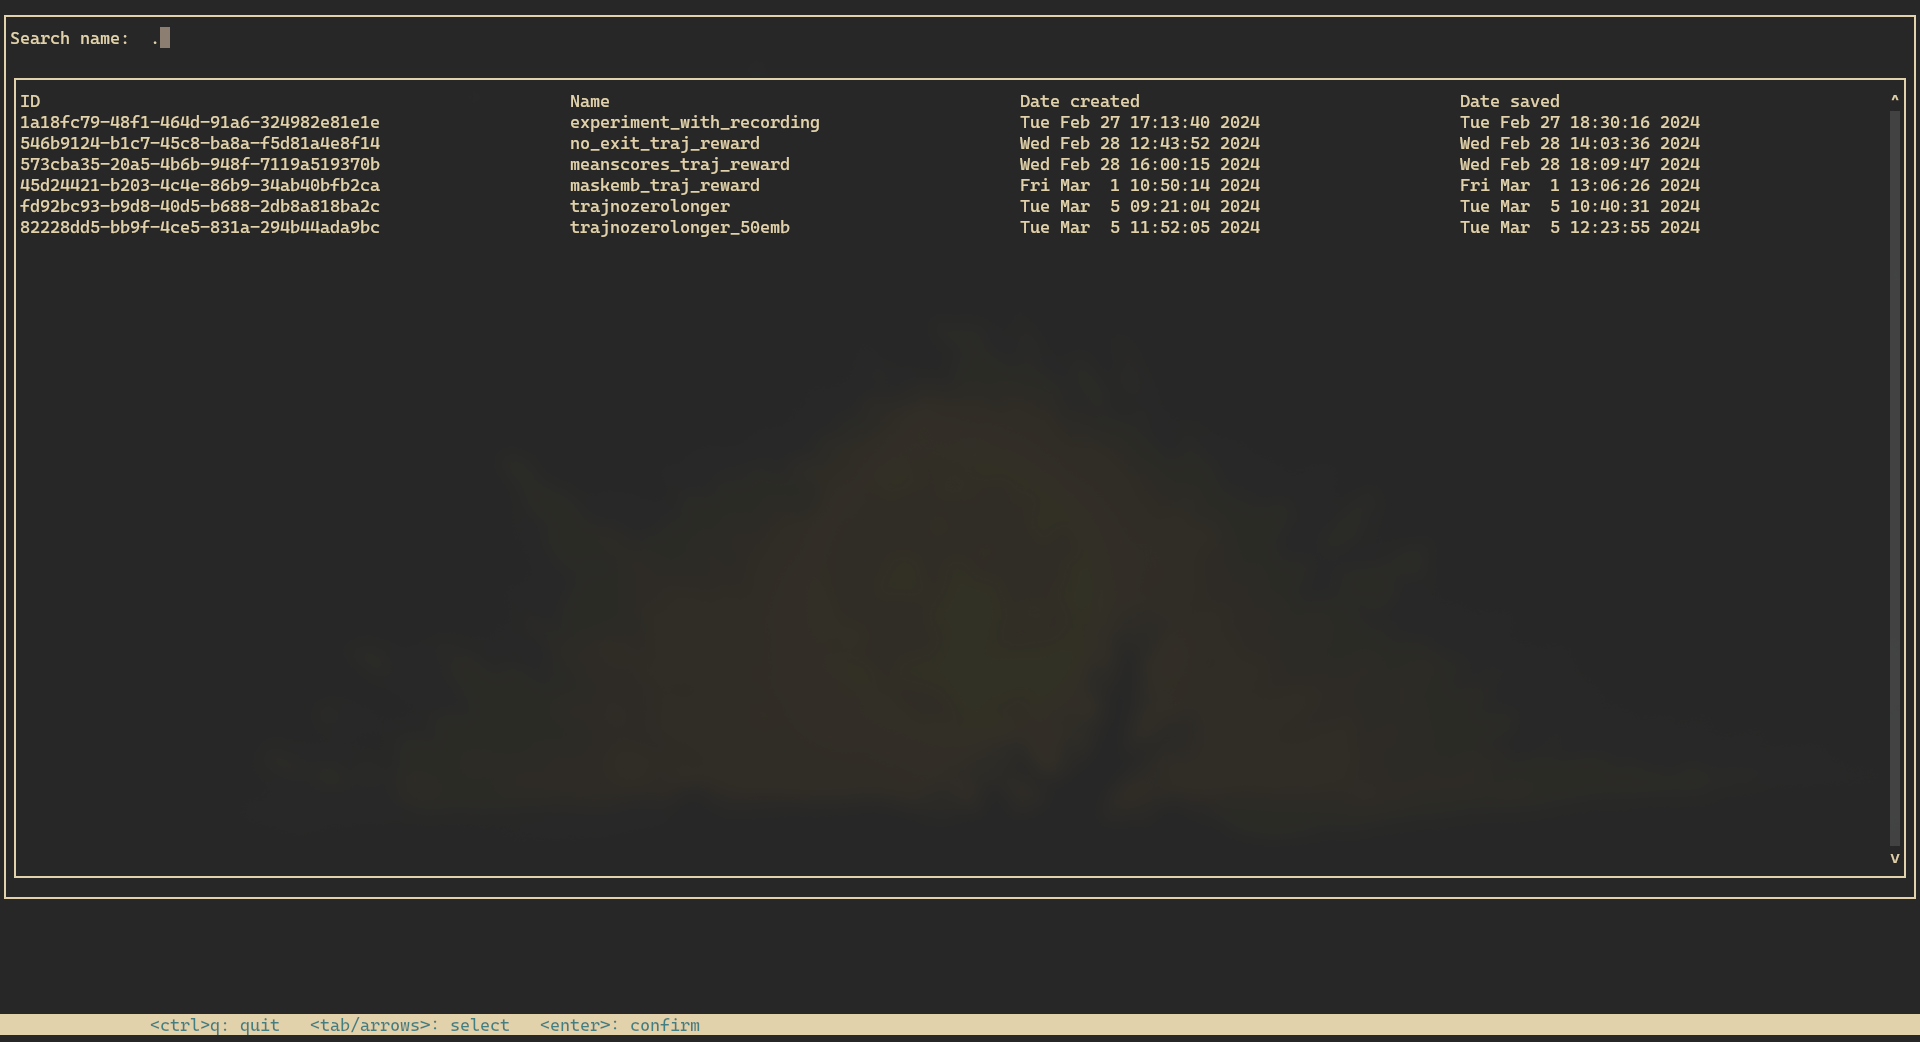
\includegraphics[width=0.90\textwidth]{tmt_search.png}
   \end{figure} 
  \end{frame}
  \begin{frame}{TMT: the TUI interface}
   \begin{figure}
    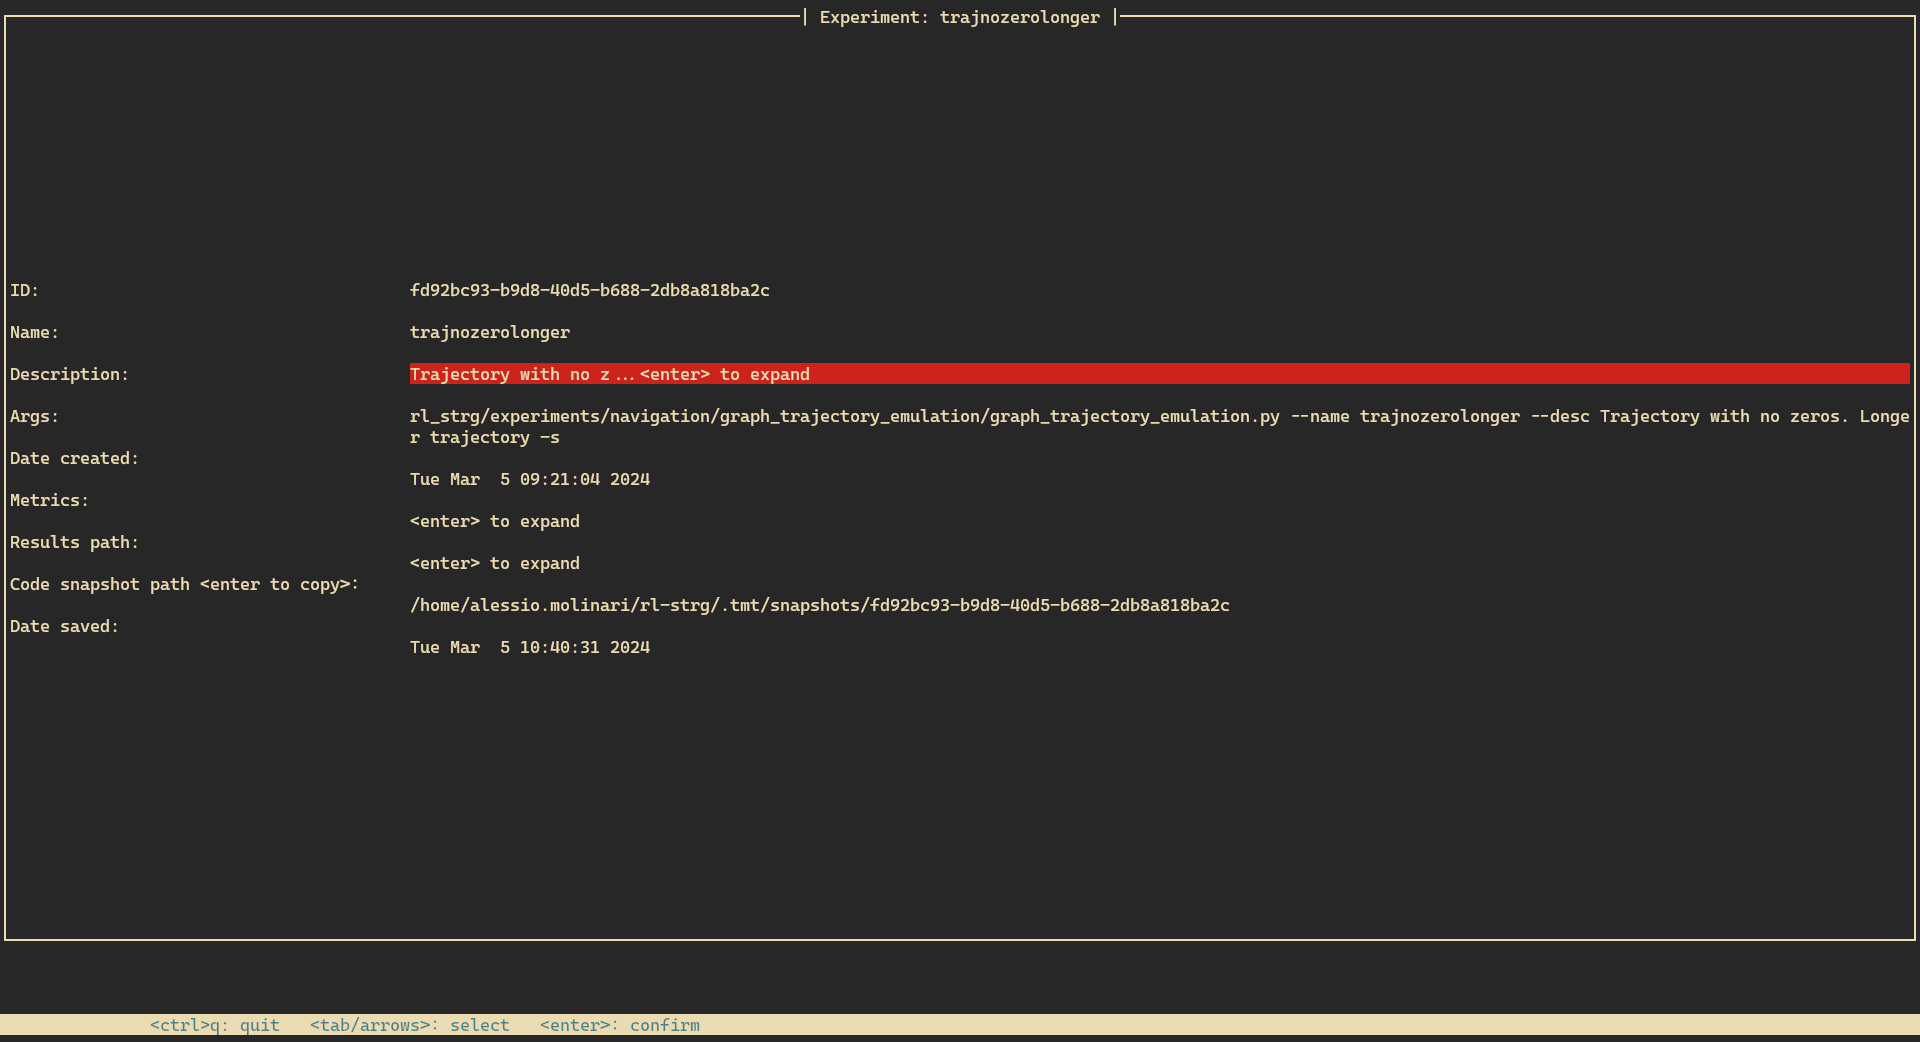
\includegraphics[width=0.90\textwidth]{detail_tui.png}
   \end{figure} 
  \end{frame}
  \begin{frame}[fragile]{TMT: loading from code}
    \begin{minted}[highlightlines={4,6,10,13}]{python3}
      from tmt import TmtManager

      manager = TmtManager()
      manager.set_entry_by_id('example')

      for name, path in manager.results_paths():
          with open(path, 'rb') as f:
              res = pickle.load(f)

      for name, res in manager.load_results():
          print(res.mean())

      for name, val in manager.get_metrics():
          print(f"{name}: {val}")
    \end{minted}
  \end{frame}

  \section{\texttt{tmt} flaws, aka I might need your help} 
  \begin{frame}{TMT: flaws and issues}
    \texttt{tmt} works and I use it more or less regularly, even today.
    However:
    \begin{itemize}
      \item since I finished my PhD, I don't really run so many experiments;
      \item I've been caught up in other open source projects;
      \item as a result, haven't been working on it for a while.
    \end{itemize}
  \end{frame}
  \begin{frame}{TMT: flaws and issues}
    Mostly:
    \begin{itemize}
      \item the TUI is cool, but a CLI would be more practical;
      \item accessing experiments (e.g., last run) should be more straight forward;
      \item \texttt{TmtManager} should be able to deal wth more than one experiment;
      \item probably more;
    \end{itemize} 
  \end{frame}
  \begin{frame}{Call for contributions}
    Contributing to open source is cool:
    \begin{itemize}
      \item you make the software you use your own \emoji{technologist}
      \item you get internet points \emoji{mage}
      \item you get resume points \emoji{office-worker}
      \item \tiny{you get to deal with strangers that ask you all kinds of weird stuff on your github issues \emoji{star-struck}}
    \end{itemize}
    \texttt{tmt} is a small project and it might be a good place to start :)
  \end{frame}
  \begin{frame}{Call for contributions}
    Sometimes it can be scary to publish or contribute code, because we think it's not good enough, or it'll be 
    judged harshly. But we all write bad code, and that's fine.
  \end{frame}


  {
    \setbeamertemplate{background}{
        \includegraphics[width=\paperwidth,height=\paperheight]{Background1.png}
  }
    {
      \begin{frame}
          \centering
           \Large Thank you! \emoji{waving-hand} \\ 
           \small Questions? \emoji{person-raising-hand}
      \end{frame}
    }
  }

\end{document}
